\documentclass{iopconfser}

\usepackage{float}
\usepackage{graphicx}
\usepackage{subcaption}
\usepackage[automake]{glossaries-extra}
\usepackage{ragged2e}
\usepackage[export]{adjustbox}
\usepackage{mathtools}
\usepackage{setspace}
\onehalfspacing
% \makeglossaries

\setabbreviationstyle[acronym]{long-postshort-user}
\glssetcategoryattribute{acronym}{nohyperfirst}{true}
\setabbreviationstyle{short-nolong}
\makeglossaries

% --------------------
% ---- Glossaries ----
% --------------------
\newglossaryentry{asyncio}{name=Asyncio, description={A Python library for asynchronous code.}}
\newglossaryentry{stim}{name=STIM300, description={A MEMS-based \gls{imu}}}
\newglossaryentry{f9p}{name=F9P, description={A Global Navigation Satellite System (GNSS) receiver manufactured by u-blox.}}

% --------------------
% ----- Acronyms -----
% --------------------
\newacronym{asv}{ASV}{Autonomous Surface Vehicle}
\newacronym{dolp}{DoLP}{Degree of Linear Polarization}
\newacronym{aolp}{AoLP}{Angle of Linear Polarization}
\newacronym{sitaw}{SITAW}{Situational Awareness}
\newacronym{poe}{PoE}{Power over Ethernet}
\newacronym{pps}{PPS}{Pulse Per Second}
\newacronym{cpfa}{CPFA}{Color-Polarization Filter Array}
\newacronym{utc}{UTC}{Coordinated Universal Time}
\newacronym{imu}{IMU}{Inertial Measurement Unit}
\newacronym{tov}{TOV}{Time of Validity}
\newacronym{tm2}{TM2}{Time mark data}
\newacronym{gnss}{GNSS}{Global Navigation Satellite System}
\newacronym{ptp}{PTP}{Precision Time Protocol}

% \glsaddall
% \makenoidxglossaries

% \glsunset{cpu}
\glsunset{gnss}
\glsunset{imu}
\glsunset{tm2}
\glsunset{utc}

% --------------------
% ----- Shortcuts ----
% --------------------


\addbibresource{mylib.bib}
 

\begin{document}

\title{AI Powered Mini Ferries, the Future of Urban Transportation or Yet Another Hype?}

\section*{<<MilliAmpere 2>>, the new research ship from NTNU, gives us sneak peak of how bridges might become obsolete in future cities.}

\begin{figure}[H]
    \centering
    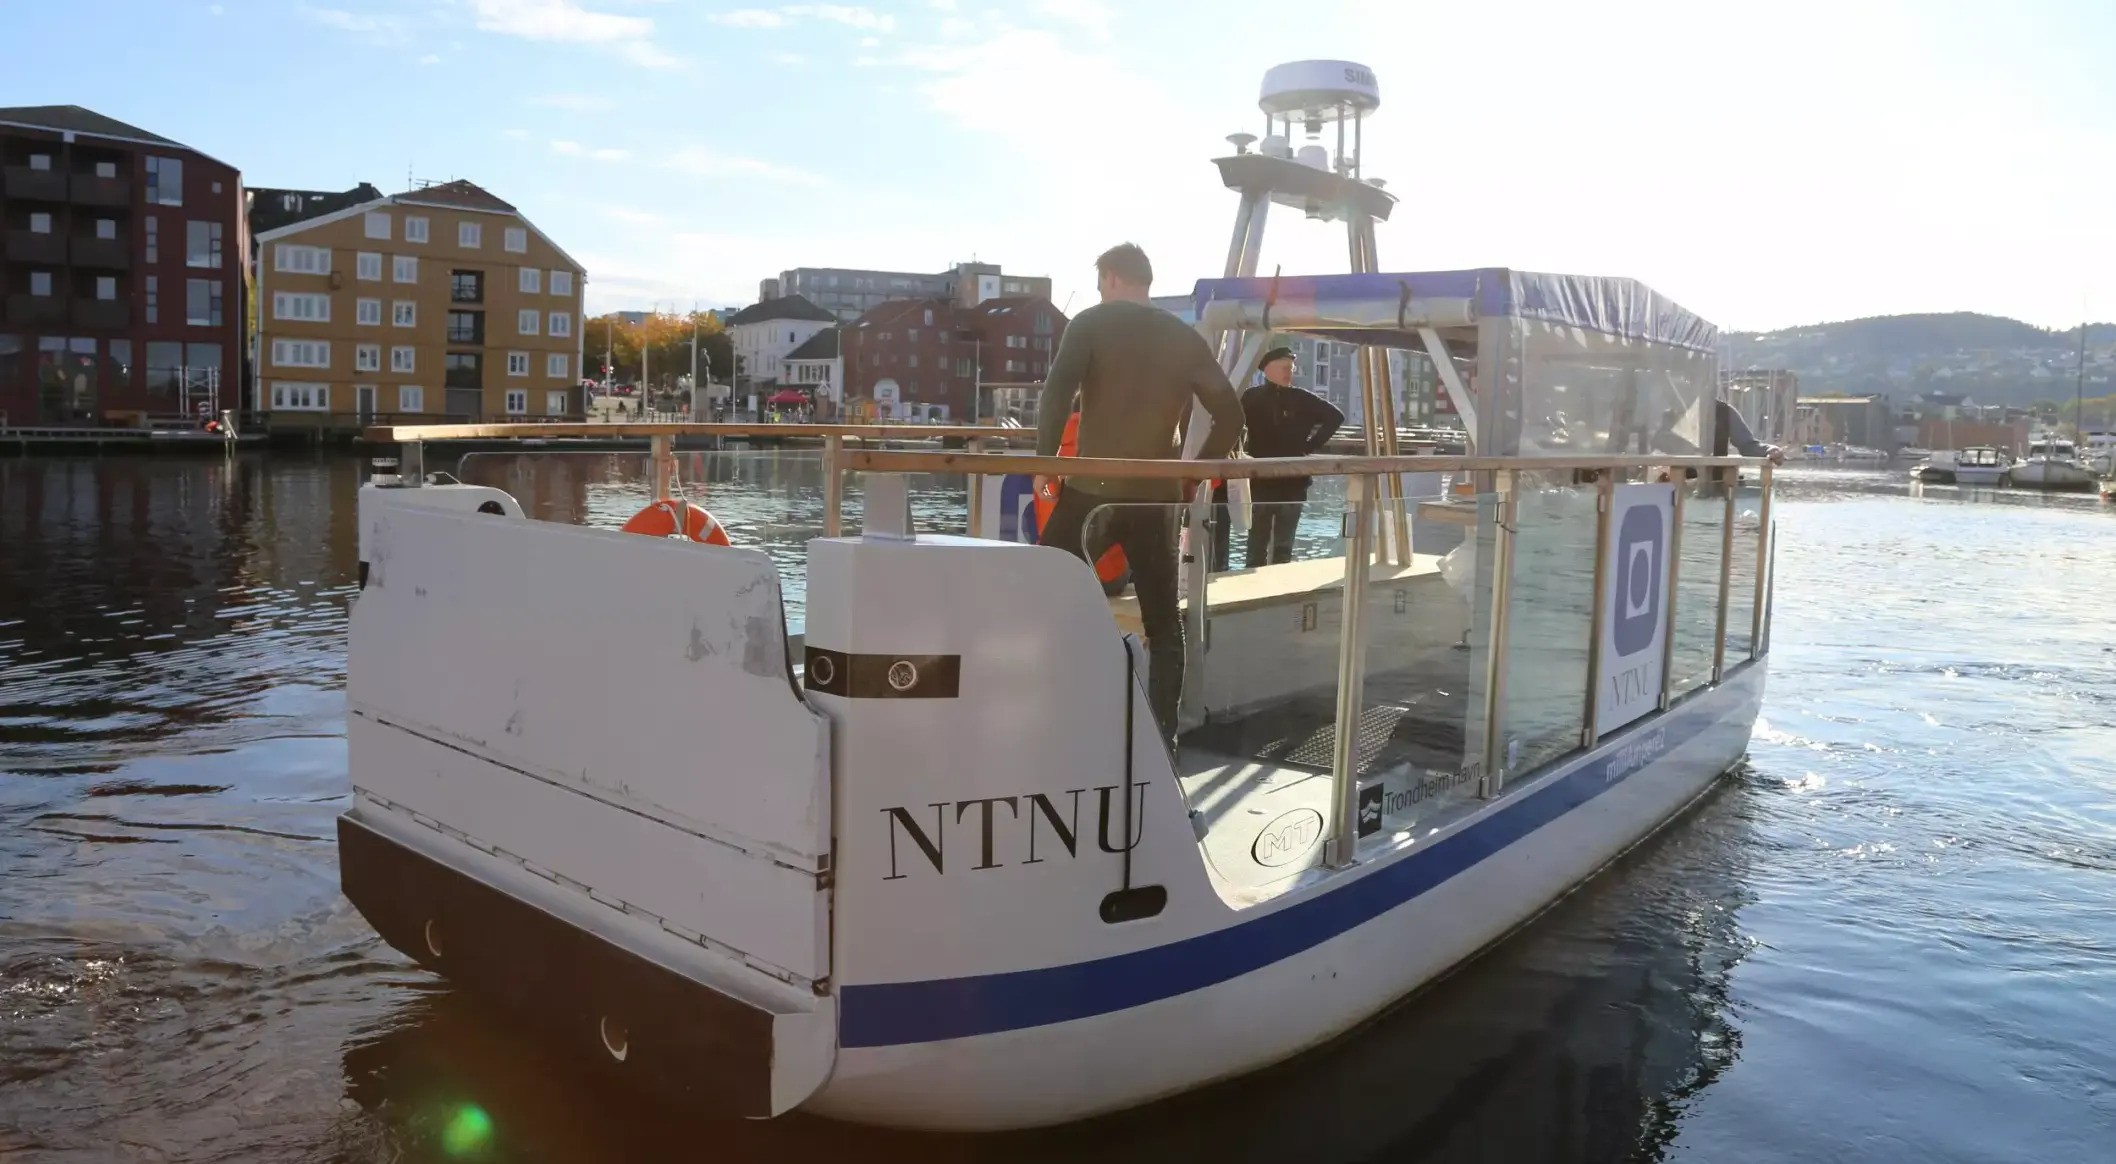
\includegraphics[width=\textwidth]{figures/milliampere.jpg}
    \caption{MilliAmpere 2 driving autonomously in Trondheim harbour \cite{hauglandDetSomHar2022}.}
\end{figure}

\section*{Artificial Intelligence in Autonomous Vehicles}
The word AI gets thrown around often, so let's clarify what AI means in this context.
As an experienced driver, you generally don't have to think a lot when driving a car.
You just have to stay in your lane, keep a safe distance from other vehicles, and follow the speed limit.
A modern car, with adaptive cruise control and lane-keeping assist, can already do most of these things.
These things would not be called AI but rather advanced automation, where a human has defined all the rules for what to do.

However, when something unexpected happens, you, as a driver, must react quickly and make the right decision.
This ability to react to new and unexpected situations is what is currently missing in autonomous vehicles, and this is what we refer to as AI when talking about autonomous vehicles.
The problem can be broken into three successive parts:
\begin{enumerate}
    \item Detecting that something unexpected is happening.
    \item Interpreting what is happening.
    \item Acting accordingly.
\end{enumerate}




\section*{Ferries VS Cars}
Autonomous cars seem to always be a couple of years away, yet they never seem to arrive.
Billions of dollars have been invested into their development, but the technology is still not ready for widespread use.
Why is the development of autonomous ferries any different?

When we start deploying autonomous vehicles, either cars or ferries, there will be a transition period where a human operator monitors each car and can take control if needed.
For autonomous cars, the human operator needs to be behind the wheel at all times to react quickly enough and avoid accidents.
Ferries, however, are a different story.
They move significantly slower than cars, have a better overview, cannot cause congestion, and do not have to deal with pedestrians like road vehicles.
An autonomous ferry, therefore, only needs to detect that something unexpected is happening and can then just alert the human operator to take control if required.
With all the extra time, the human operator does not even need to be on board the ship but can instead be located remotely, look at the video feed from the ship, and control the ferry like an online video game.
This makes it possible for one human operator to monitor multiple ferries at the same time, making the operation cheaper and more efficient.
Being a stuck passenger on a ferry waiting for a remote human operator to take control might be annoying, but it is not dangerous.
This makes the transition to fully autonomous ferries much more gradual and less risky than cars.
Being located on the water with a line of sight to infrastructure on land also makes it easier to deploy 5G networks that can be used to reliably operate the ferries remotely.

\section*{MilliAmpere 2}
MilliAmpere 2 is NTNU's new research ferry, which is currently being used to develop autonomous ferries.
With eight cameras, multiple lidars, and a radar, it provides information about its surroundings and including how far away other objects are.
Researchers have developed systems using this data to enable MilliAmpere 2 to navigate across the harbor autonomously, avoiding other boats.
To ensure safety, they have programmed MilliAmpere 2 to have a conservative approach, halt operations when unexpected circumstances are detected and alert the human operator if the situation does not solve itself.
Even though the ferry can be controlled remotely, a human operator is currently always on board to take control if needed.
Residents of Trondheim have already had the privilege of experiencing the convenience of MilliAmpere 2, with rides across the harbor.

It is still the early days for autonomous ferries, but the technology appeart to be improving rapidly.
In the future, fully autonomous ferries might make the commute between different parts of the city significantly easier.
It only remains to be seen whether the development of autonomous ferries takes as long as for autonomous cars, but currently, the problem seems to be much easier to solve.


\newpage
\title{Reflections}
This text is aimed at the part of the general public that is slightly skeptical towards autonomy, with the goal of convincing them that autonomous ferries might be an easier problem to solve than autonomous cars.

\section*{Me the Writer}
Acknowledging my position in relation to the topic is a good place to start before analyzing the target audience.
As I am taking a PhD in autonomous systems, I'm hopefully more knowledgeable about the technology than the average person and should be aware of the vocabulary and concepts I use to explain it.
While researchers might be very pedantic about details and technicalities, it is important to note that to engage with a broader audience, it is often better to avoid the technicalities and focus on the message \cite{kulykPeopleWantReassurance2023}.

As a researcher in the field, I'm more positive toward autonomous technology than the average person, but knowing how hard it is to implement seemingly simple features makes me believe that the technology is still far away from being ready for widespread use.
I'm also a bit skeptical about autonomous ferries for people, as they have many more safety requirements than ferries for cargo transport.
However, I do not mention this in the text, as it is not relevant to the message I want to convey.

\section*{The Target Audience}
With AI and autonomy being a hot topic in the news, I think most people are familiar with the concept and have some kind of opinion on it.

In terms of competence, the text is aimed at people familiar with autonomous vehicles but without any expertise.
The text tries to avoid using complex language, and the technical terms, like "lidar," are not necessary to understand to get the text's message.
I assume that the reader is familiar with driving a car and uses several comparisons and metaphors related to driving.
This can effectively communicate ideas as we can leverage the reader's knowledge and sentiment from another topic, as was discussed in the third lecture of thie course \cite{gustafssonCognitiveLinguisticsScience2024}.
However, these metaphors might make the text less adapted to young people and people without a driver's license.

Convincing skeptics is hard, and convincing optimists is unnecessary, so the text is aimed at the people in the lower middle segment of the public in terms of how positive they are towards autonomous vehicles.
I start with the title by framing it as an open question to make the reader curious about the topic and avoid appearing naive.
While optimistic, the text acknowledges that the technology is still in its early days and that we don't yet know how long it will take.
However, the text presents it as a question of "when" rather than "if" autonomous ferries will be a reality, which is a subtle way of convincing the reader that it will happen.

\begin{figure}[H]
    \centering
    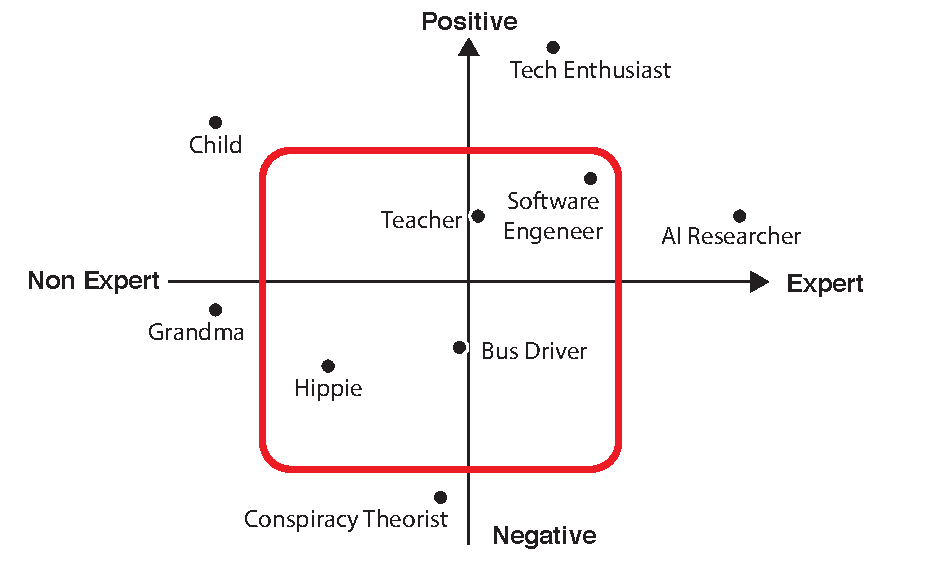
\includegraphics[width=.8\textwidth]{figures/overview.pdf}
    \caption{Visualization of the target audience, marked in red, for this text.
        The occupations in the figure are mostly based on my own assumptions and are quite stereotypical.}
\end{figure}

\section*{How Agency is Framed}
Framing plays a big role in how a text is received \cite{lakoffWhyItMatters2010}\cite{gustafssonCognitiveLinguisticsScience2024}.
We often see language that frames autonomous systems as having a high degree of agency, which can be misleading and make people skeptical of the technology.
For instance, it is fairly common to use words like "understand," "observe," "decide," and "think" rather than more passive synonyms when talking about autonomous systems.
Actors with an agency we don't understand can be scary, like monsters or aliens.
"The autonomous car observed the pedestrian and decided to stop" sounds a lot more ominous than "The autonomous car detected the pedestrian and stopped."
Similar to how conservatives have been successful at building up frames that suit their interest \cite{lakoffWhyItMatters2010}, I believe media have framed autonomous systems as some spectacular technology that can think and act on its own.
This is more intriguing and generates more clicks, and might be why we find articles like the one in Dagbladet presenting Milliampere 2 and still talks about killer robots \cite{fjeldSelvstyrtFerjeVekker2022}.
Since how we frame AI impacts how people perceive it \cite{bingamanSiriShowMe2021}, I think it is important for researchers to be aware of this and try to frame them in a more passive way.
In the text where I talk about the three steps needed for an autonomous system to react to an unexpected event, I, therefore, used "detect," "interpret," and "act" instead of "observe," "understand," and "decide."

I believe that making people trust automated machines is a lot more difficult than making them trust other people.
People generally do not question the ability of the bus driver to drive the bus, but they might question the ability of an autonomous bus to drive itself.
With this in mind I try to fraim the automated machines as passive agents that is either programmed by a human or controlled by a human.
One practical way I do this is by consistently saying "human operator" rather than just "operator" and sayin that "researchers have programmed it", rather that "it is programmed".
Hopefully, the reader will subconsciously trust the researcher and operator and transfer that trust to the autonomous system.
Reassuring the reader that safety is a top priority is also a way to build trust \cite{kulykPeopleWantReassurance2023}.

\section*{Acknowledging Other Narratives}
Where framing is about how we present information in a way that benefits our standpoint, narratives are about the overall story we tell, and it can be a powerful tool to communicate science to the public \cite{dahlstromUsingNarrativesStorytelling2014}.
In this text I try to sell the story that autonomous ferries is a realistic and safe technology that is not too far away.
A big issue with this is that the same story has been told about autonomous cars for the last 20 years, which probably makes people skeptical about autonomous ferries as it is like the boy who cried wolf.
To handle this, I acknowledge this similarity and focus on explaining why ferries are different from cars to separate the two narratives.

Regarding the ethical use of narratives that Dahlström talks about \cite{dahlstromUsingNarrativesStorytelling2014}, the narrative presented here aims at informing the public but acknowledges that the technology is still in its early days and that we don't yet know if autonomous ferries will be successful.
Since I'm personally a bit sceptical towards its use to transport humans I could have mentioned this to keep my full integrity, but I believe it would have distracted to much from the message of the text.


\section*{Benefit to Society}
In this text I targeted scepticisom towards the possibility of autonomous ferries, and does not dive into the topic of whether or not the autonomous ferries is a good idea over all.
I believe automation of labor will have a positive impact on society, but it will require policies to avoid large increases in unemployment and social inequality.
A discussion on these implications of automation is certainly interesting and important, but I think it is generally a good idea to separate that discussion from whether or not different types of automation are technically possible.

Green public transport is also one part of automation that is pretty uncontroversial, and I think most people would agree that it is a good idea.
It is still worth noting that it is part of a culture clash between rural people driving diesel trucks and urban people drinking soy lattes.

\section*{Contribution to the Discusion}
There have been quite a few news articles covering the relase of MilliAmpere 2
\cite{fjeldSelvstyrtFerjeVekker2022}
\cite{andreassenNorskSelvkjorendeFerje2022a}
\cite{tranaHaperSmaOg2019}
\cite{okstadTilSommerenVil2020}
\cite{auneDetteHarAldri2022}
\cite{killingbergTrengerMillionerBli2022}
\cite{riestoSelvkjoRendeByferje2022}
\cite{hauglandDetSomHar2022}
\cite{skoglundAvtalenKlarOm2024}
\cite{hauganSelvkjorendeFergeForst2022}
All of these articles were quite similar in that they gave a brief presentation of the ferry with a focus on it being new technology.
Compared to the other news articles, the text I have written is more focused on explaining how autonomous ferries are different from autonomous cars, which is not something that has been properly covered in the other news articles.
Some other viewpoints I considered taking was on why transporting cargo might be easier than transporting people, if this type of technology is economically viable and if it is a good idea to have autonomous ferries in the first place.


\section*{Thanks for a nice semester, enjoy the summer!}

\pagebreak
\section*{Use of Language Models}
I wrote this text in VS Code where GitHub Copilot sometimes suggests completions for the text, which I occasionally use to speed up the writing process.
I did have a couple of conversations with GPT-4o, notably to learn more about the distinction between frames and narratives, but it did not contribute significantly to the text.
The final text was passed through Grammarly to fix spelling mistakes and get suggestions on how to improve the language.
All the content in this exam is my own.

\printbibliography

\end{document}